\documentclass[a4paper, 12pt]{article}

\usepackage[ a4paper,
 total={170mm,257mm},
 left=20mm,
 top=20mm,]{geometry}

\usepackage{cmap}
\usepackage[T2A]{fontenc}
\usepackage[utf8]{inputenc}
\usepackage[english, russian]{babel}

%Графика
\usepackage{graphicx}
\usepackage{float}%"Плавающие" картинки
\usepackage{wrapfig}%Обтекание фигур (таблиц, картинок и прочего)
\graphicspath{{./images/}}

% Математика
\usepackage{amsmath,amsfonts,amssymb,amsthm,mathtools} 

%Title Page
\title{ЛАБОРАТОРНАЯ РАБОТА № 2 \\
Моделирование механических систем
}
\author{Вариант 11 \\ Машуров Владимир БПМ-19-3}

\setcounter{page}{0}

\begin{document}
\maketitle
\thispagestyle{empty}
\newpage
\tableofcontents

\section{Моделирование механической системы масса-пружина}

Дана система:

\begin{equation}
M\ddot{x} + B\dot{x} + kx = f(t)
\label{СистемаСБлокомНаПружинеИДемпфером}
\end{equation}

Где $f(t)$ - входное воздействие, $x(t)$ - выходное воздействие.
 
\textbf{Задание 1.1 } \\
Применив преобразование Лапласа (с нулевыми начальными условиями) найдите передаточную функцию модели: $ G(s) = \frac{X(s)}{F(s)} $ 

Найдём соотношение из которого получим G(t):


$$M\ddot{x}(t) + B\dot{x}(t) + kx(t) = f(t) \; \; \; \frac{d}{dt} = \lambda $$

$$ M\lambda^2x(t) + B\lambda x(t) + kx(t) = f(t) $$

$$ (M\lambda^2 + B\lambda + k)x(t) = f(t) $$

$$ \frac{x(t)}{f(t)} = \frac{1}{M\lambda^2 + B\lambda + k} $$

Отсюда

$$ G(s) = \frac{X(s)}{F(s)} = \mathcal{L} \bigg( \frac{x(t)}{f(t)} \bigg) = \frac{\mathcal{L}(\tilde{x}(t))}{\mathcal{L}(\tilde{f}(t))} = $$
$$ = \frac{\mathcal{L}(1)}{\mathcal{L}(M\lambda^2 + B\lambda + k)} =  \frac{1}{s} \cdot \frac{s}{M\lambda^2 + B\lambda + k} = \frac{1}{M\lambda^2 + B\lambda + k} $$

\textbf{Задание 1.2 } \\
Перепишите уравнение \ref{СистемаСБлокомНаПружинеИДемпфером} в форму вход-состояние-выход.

$$M\ddot{x}(t) + B\dot{x}(t) + kx(t) = f(t) $$ 

Разделим всё на $M$ и заменим переменные следующим образом, для удобства: $f = U$ и $x = y$. Получим 

$$ \ddot{y} + \frac{B}{M}\dot{y} + \frac{k}{M}y = \frac{1}{M}U $$

Составим систему:

$$ \begin{cases}
x_1 = y \\
x_2 = \dot{y} + \frac{B}{M} y
\end{cases} $$

Продифференцируем оба равенства по $t$

$$ \begin{cases}
\dot x_1 = \dot y = x_2 - \frac{B}{M} y \\
\dot x_2 = \ddot y +\frac{B}{M} \dot y = \frac{1}{M} U - \frac{k}{M} y = \frac{1}{M} U - \frac{k}{M} x_1
\end{cases} $$

Мы пришли к форме вход-состояние-выход. Обратим замену переменных:

$$ \begin{cases}
\dot \pi_1 = \pi_2 - \frac{B}{M} x \\
\dot \pi_2 = \frac{1}{M} f - \frac{k}{M} \pi_1
\end{cases} $$

Легко заметить, что:

\[
A = \begin{bmatrix}
-\dfrac{k}{M} & 1\\ \\
-\dfrac{B}{M} & 0 
\end{bmatrix}	
\;
B = \begin{bmatrix}
0 \\
-\frac{1}{M}
\end{bmatrix}
\;
C = \begin{bmatrix}
1 & 0
\end{bmatrix}	
\]

\textbf{Задание 1.3 } \\
Составьте структурную схему моделирования, опираясь на уравнение \ref{СистемаСБлокомНаПружинеИДемпфером} и результат, полученный в Задании 2.

$$M\ddot{x}(t) + B\dot{x}(t) + kx(t) = f(t) \; \; \; |:M $$

$$\ddot{x}(t) + \frac{B}{M}\dot{x}(t) + \frac{k}{M}x(t) = \frac{1}{M} f(t) $$

$$ \ddot{x}(t) = \frac{1}{M} f(t) - \frac{k}{M}x(t) - \frac{B}{M}\dot{x}(t) \; \; \; |\frac{d}{dt} = \lambda$$

$$ \lambda^2 x(t) = \frac{1}{M} f(t) - \frac{k}{M}x(t) - \frac{B}{M} \lambda x(t) \; \; \; |:\lambda^2$$

$$ x(t) = \frac{1}{\lambda^2} \Big( \frac{1}{M} f(t) - \frac{k}{M}x(t) \Big) -\frac{1}{\lambda} \Big( \frac{B}{M} x(t) \Big) $$


Из полученного выражения можно построить структурную схему, изображенную на рисунке \ref{p:Схема1}.

\begin{figure}[h!]
	\centering
	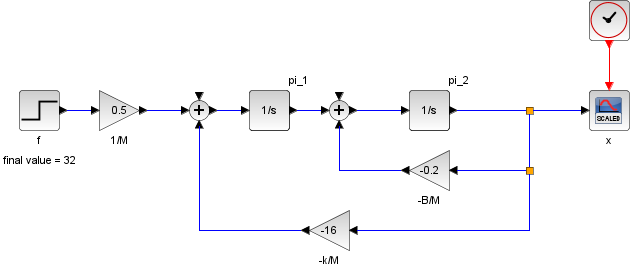
\includegraphics[scale=0.6]{scheme1-1}
	\caption{Структурная схема моделирования механической системы масса-пружина }
	\label{p:Схема1}
\end{figure}

\textbf{Задание 1.4 } \\
Для системы находящейся в состоянии покоя, в момент времени $t = 0$ прикладывается постоянная сила $f(t) = 32$ Н. Рассматриваемая система имеет массу $2$ кг и жесткость пружины $32$ кг / с2. Коэффициент демпфирования B можно отрегулировать для получения желаемого отклика. Выполните моделирование в пакете
MATLAB/Simulink (Scilab).

Получим схему на рисунке \ref{p:Схема2} и графики на рисунке \ref{p:Графики1}.

\begin{figure}[h!]
	\centering
	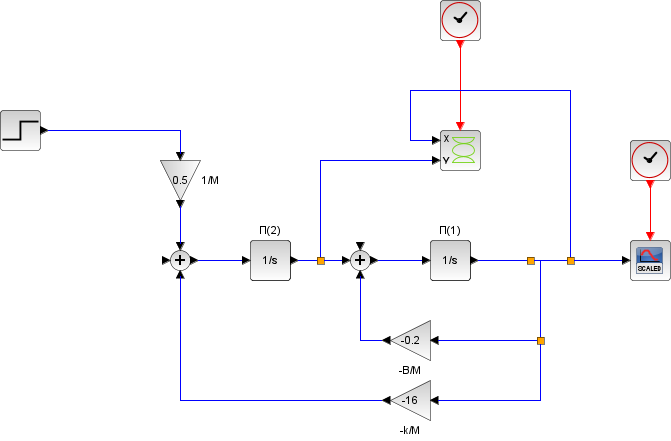
\includegraphics[scale=0.6]{scheme1-2}
	\caption{Структурная схема моделирования механической системы масса-пружина с заданными условиями }
	\label{p:Схема2}
\end{figure}

\begin{figure}[h!]
	\centering
	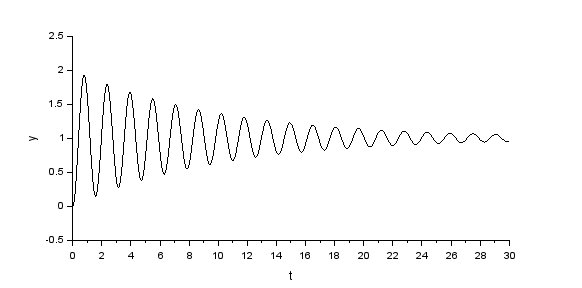
\includegraphics[scale=0.8]{graph1-1}
	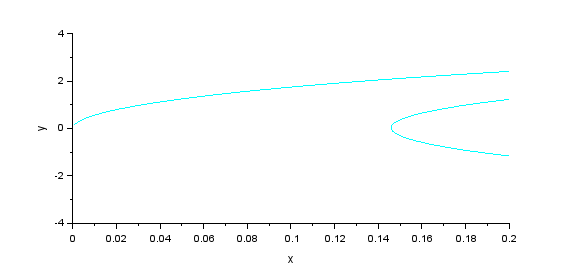
\includegraphics[scale=0.8]{graph1-2}
	\caption{График изменения положения груза во времени (сверху) и график зависимости скорости от положения системы (снизу) }
	\label{p:Графики1}
\end{figure}

\newpage

\section{Моделирование математического маятника}
Дана система математического маятника, колебания которой описываются уравнением \ref{eq:МатематическийМаятник}.
\begin{equation}
\ddot{\theta} + \frac{b}{M}\dot{\theta} + \frac{g}{l}\sin\theta = 0
\label{eq:МатематическийМаятник}
\end{equation}

\textbf{Задание 2.1} \\ Перепишите уравнение в форму вход-состояние-выход.

Если мы допустим, что колебания достаточно малы, т. е. $\theta \to 0$, тогда можно представить $\sin\theta = \theta + o(\theta)$, где $o(\theta)$ - бесконечно малая функция, а значит уравнение \ref{eq:МатематическийМаятник} можно переписать в следующем виде:

$$ \ddot{\theta} + \frac{b}{M}\dot{\theta} + \frac{g}{l}\theta = 0 $$ 

Откуда получим матрицы для представления в форме вход-состояние-выход:

\[
A = \begin{bmatrix}
-\dfrac{B}{M} & 1\\ \\
-\dfrac{g}{l} & 0 
\end{bmatrix}	
\;
B = \begin{bmatrix}
0 \\
0
\end{bmatrix}
\;
C = \begin{bmatrix}
1 & 0
\end{bmatrix}	
\]

\textbf{Задание 2.2} \\
Составьте структурную схему моделирования, опираясь на уравнение (1) и результат, полученный ранее

\textbf{Задание 2.3} \\ Выполните моделирование в пакете MATLAB/Simulink (Scilab). Исходные
данные. Масса смещена от положения равновесия на $0.5$ радиана в момент времени $t = 0$. Масса $m = 0.5$ кг, длина стержня $l = 0.6$ м а ускорение свободного падения - $9,81$ м
/ с2. Будем рассматривать два случая коэффициента трения: 
\begin{enumerate}
\item $B =0.05$ кг-с/м;
\item $B =0.4$ кг-с/м;
\end{enumerate}


\begin{figure}[h!]
	\centering
	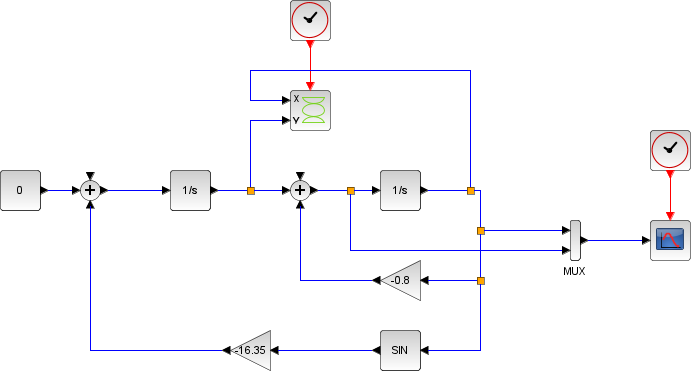
\includegraphics[scale=0.6]{scheme2}
	\caption{Структурная схема моделирования механической системы математического маятника с заданными условиями }
	\label{p:Схема3}
\end{figure}

Для решения задач построим схему на рисунке \ref{p:Схема3}. Проведём симуляцию и получим графики зависимостей, которые можно увидеть на рисунках \ref{p:Графики2-1} и \ref{p:Графики2-2}.

\begin{figure}[h!]
	\centering
	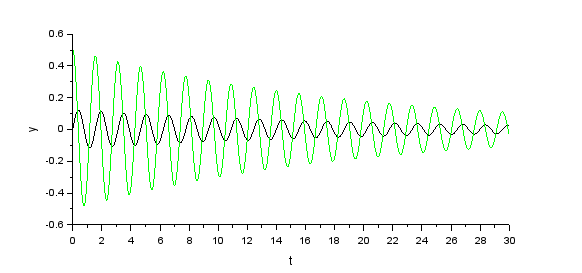
\includegraphics[scale=0.8]{graph2-1}
	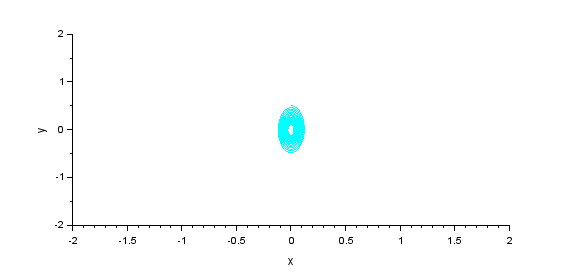
\includegraphics[scale=0.8]{graph2-2}
	\caption{Графики изменения угла и скорости со временем (сверху) и зависимости скорости от смещения (снизу) для $B = 0.05$ кг-с/м }
	\label{p:Графики2-1}
\end{figure}

\begin{figure}[h!]
	\centering
	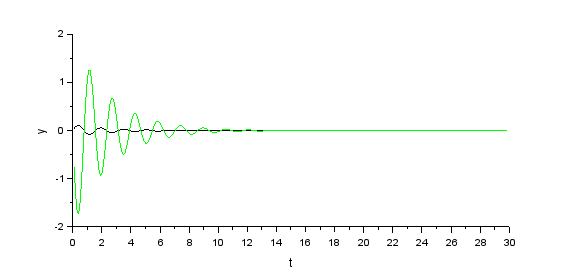
\includegraphics[scale=0.8]{graph2-3}
	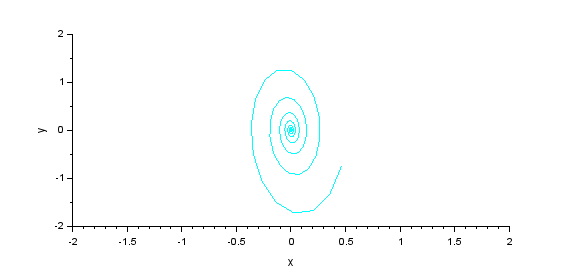
\includegraphics[scale=0.8]{graph2-4}
	\caption{Графики изменения угла и скорости со временем (сверху) и зависимости скорости от смещения (снизу) для $B = 0.4$ кг-с/м  }
	\label{p:Графики2-2}
\end{figure}

\end{document}